\documentclass[a4paper,14pt]{extarticle}

\newcommand{\stend}{\textbf{Wb-demo-kit v.2}}

% Путь до папки с общими шаблонами
\newcommand{\pathToCommonFolder}{/home/denilai/Documents/repos/latex/Common}

% Название работы в титуле
\newcommand{\workname}{Отчет по практическим работам 9-12}
% Название дисциплины в титуле
\newcommand{\discipline}{Технологические основы Интернета вещей}
% Название кафедры в титуле
\newcommand{\kafedra}{Кафедра Математического обеспечения и стандартизации информационных технологий}
% Тема работы в титуле
\newcommand{\theme}{}
% Должность преподавателя в титуле
\newcommand{\rang}{ассистент}

% ФИО студента в титуле
\newcommand{\studentfio}{К.~Ю.~Денисов}%\\Д.~Н.~Федосеев\\А.~М.~Сосунов}\\%К.~Ю.~Денисов\\%И.~А.~Кремнев
% ФИО преподавателя в титуле
\newcommand{\teacherfio}{Ю.~А.~Воронцов}


\usepackage{tabularx}


\usepackage{booktabs}
\newcolumntype{b}{X}
\newcolumntype{s}{>{\hsize=.5\hsize}X}
\newcommand{\heading}[1]{\multicolumn{1}{c}{#1}}

% установка размера шрифта для всего документа
%\fontsize{20pt}{18pt}\selectfont
\usepackage{extsizes} % Возможность сделать 14-й шрифт

% Вставка заготовки преамбулы
% Этот шаблон документа разработан в 2014 году
% Данилом Фёдоровых (danil@fedorovykh.ru) 
% для использования в курсе 
% <<Документы и презентации в \LaTeX>>, записанном НИУ ВШЭ
% для Coursera.org: http://coursera.org/course/latex .
% Исходная версия шаблона --- 
% https://www.writelatex.com/coursera/latex/5.3

% В этом документе преамбула

% Для корректного использования русских символов в формулах
% пакеты hyperref и настройки, связанные с ним, стоит загуржать
% перед загрузкой пакета mathtext



% поддержка русских букв
% кодировка шрифта
%\usepackage[T2A]{fontenc} 
\usepackage{pscyr}

% использование ненумеровонного абзаца с добавлением его в содержаниеl

\newcommand{\anonsection}[1]{\section*{#1}\addcontentsline{toc}{section}{#1}}
\newcommand{\sectionunderl}[1]{\section*{\underline{#1}}}


% настройка окружения enumerate
\usepackage{enumitem}
\setlist{noitemsep}
\setlist[enumerate]{labelsep=*, leftmargin=1.5pc}

\usepackage{hyperref}

% сначала ставить \usepackage{extsizes} % Возможность сделать 14-й шрифт
% для корректной установки полей вставлять преамбулу следует в последнюю очередь (но перед дерективой замены \rmdefault)
\usepackage[top=20mm,bottom=25mm,left=35mm,right=20mm]{geometry} % Простой способ задавать поля

\hypersetup{				% Гиперссылки
	unicode=true,           % русские буквы в раздела PDF
	pdftitle={Заголовок},   % Заголовок
	pdfauthor={Автор},      % Автор
	pdfsubject={Тема},      % Тема
	pdfcreator={Создатель}, % Создатель
	pdfproducer={Производитель}, % Производитель
	pdfkeywords={keyword1} {key2} {key3}, % Ключевые слова
	colorlinks=true,       	% false: ссылки в рамках; true: цветные ссылки
	linkcolor=red,          % внутренние ссылки
	citecolor=black,        % на библиографию
	filecolor=magenta,      % на файлы
	urlcolor=blue           % на URL
}

%%% Работа с русским языком
\usepackage{cmap}					% поиск в PDF
\usepackage{mathtext} 				% русские буквы в формулах
\usepackage[T2A]{fontenc}			% кодировка
\usepackage[utf8]{inputenc}			% кодировка исходного текста
\usepackage[english,russian]{babel}	% локализация и переносы
\usepackage{indentfirst}
\frenchspacing

%для изменения названия списка иллюстраций
\usepackage{tocloft}


\renewcommand{\epsilon}{\ensuremath{\varepsilon}}
\renewcommand{\phi}{\ensuremath{\varphi}}
\renewcommand{\kappa}{\ensuremath{\varkappa}}
\renewcommand{\le}{\ensuremath{\leqslant}}
\renewcommand{\leq}{\ensuremath{\leqslant}}
\renewcommand{\ge}{\ensuremath{\geqslant}}
\renewcommand{\geq}{\ensuremath{\geqslant}}
\renewcommand{\emptyset}{\varnothing}

% Изменения параметров списка иллюстраций
\renewcommand{\cftfigfont}{Рисунок } % добавляем везде "Рисунок" перед номером
\addto\captionsrussian{\renewcommand\listfigurename{Список иллюстративного материала}}

\newcommand{\tm}{\texttrademark\ }
\newcommand{\reg}{\textregistered\ }


%%% Дополнительная работа с математикой
\usepackage{amsmath,amsfonts,amssymb,amsthm,mathtools} % AMS
\usepackage{icomma} % "Умная" запятая: $0,2$ --- число, $0, 2$ --- перечисление

%% Номера формул
%\mathtoolsset{showonlyrefs=true} % Показывать номера только у тех формул, на которые есть \eqref{} в тексте.
%\usepackage{leqno} % Нумереация формул слева

%% Свои команды
\DeclareMathOperator{\sgn}{\mathop{sgn}}

%% Перенос знаков в формулах (по Львовскому)
\newcommand*{\hm}[1]{#1\nobreak\discretionary{}
{\hbox{$\mathsurround=0pt #1$}}{}}


% отступ для первого абзаца главы или параграфа
%\usepackage{indentfirst}

%%% Работа с картинками
\usepackage{graphicx}  % Для вставки рисунков
\graphicspath{{images/}{screnshots/}}  % папки с картинками
\DeclareGraphicsExtensions{.pdf,.png,.jpg}
\setlength\fboxsep{3pt} % Отступ рамки \fbox{} от рисунка
\setlength\fboxrule{1pt} % Толщина линий рамки \fbox{}
\usepackage{wrapfig} % Обтекание рисунков текстом

%%% Работа с таблицами
\usepackage{array,tabularx,tabulary,booktabs} % Дополнительная работа с таблицами
\usepackage{longtable}  % Длинные таблицы
\usepackage{multirow} % Слияние строк в таблице

%%% Теоремы
\theoremstyle{plain} % Это стиль по умолчанию, его можно не переопределять.
\newtheorem{theorem}{Теорема}[section]
\newtheorem{proposition}[theorem]{Утверждение}

\theoremstyle{plain} % Это стиль по умолчанию, его можно не переопределять.
\newtheorem{work}{Практическая работа}[part]


 
 
\theoremstyle{definition} % "Определение"
\newtheorem{corollary}{Следствие}[theorem]
\newtheorem{problem}{Задача}[section]
 
\theoremstyle{remark} % "Примечание"
\newtheorem*{nonum}{Решение}



%%% Программирование
\usepackage{etoolbox} % логические операторы

%%% Страница

%	\usepackage{fancyhdr} % Колонтитулы
% 	\pagestyle{fancy}
%   \renewcommand{\headrulewidth}{0pt}  % Толщина линейки, отчеркивающей верхний колонтитул
% 	\lfoot{Нижний левый}
% 	\rfoot{Нижний правый}
% 	\rhead{Верхний правый}
% 	\chead{Верхний в центре}
% 	\lhead{Верхний левый}
%	\cfoot{Нижний в центре} % По умолчанию здесь номер страницы

\usepackage{setspace} % Интерлиньяж
\onehalfspacing % Интерлиньяж 1.5
%\doublespacing % Интерлиньяж 2
%\singlespacing % Интерлиньяж 1

\usepackage{lastpage} % Узнать, сколько всего страниц в документе.

\usepackage{soul} % Модификаторы начертания


\usepackage[usenames,dvipsnames,svgnames,table,rgb]{xcolor}


\usepackage{csquotes} % Еще инструменты для ссылок

%\usepackage[style=authoryear,maxcitenames=2,backend=biber,sorting=nty]{biblatex}

\usepackage{multicol} % Несколько колонок

\usepackage{tikz} % Работа с графикой
\usepackage{pgfplots}
\usepackage{pgfplotstable}

% модуль для вставки рыбы
\usepackage{blindtext}

\usepackage{listings}
\usepackage{color}


% для поворота отдельной страницы. Использовать окружение \landscape
\usepackage{pdflscape} 
\usepackage{rotating} 


\definecolor{mygreen}{rgb}{0,0.6,0}
\definecolor{mygray}{rgb}{0.5,0.5,0.5}
\definecolor{mymauve}{rgb}{0.58,0,0.82}


% пример импорта файла
%\lstinputlisting{/home/denilai/repomy/conf/distributions}

\lstset{
	language=Python,
	basicstyle=\footnotesize,        % the size of the fonts that are used for the code
	numbers=left,                    % where to put the line-numbers; possible values are (none, left, right)
	numbersep=5pt,                   % how far the line-numbers are from the code
	numberstyle=\tiny\color{mygray}, % the style that is used for the line-numbers
	stepnumber=2,                    % the step between two line-numbers. If it's 1, each line will be numbered
	% Tab - 2 пробела
	tabsize=2,    
	% Автоматический перенос строк
	breaklines=true,
	frame=single,
	breakatwhitespace=true,
	title=\lstname 
}



\author{Кирилл Денисов}
\title{Лабораторная работа №1}
\date{\today}

\renewcommand{\withouttheme}{1}

%если нужна тема работы в отчете, то указать в скобках что-либо, иначе оаставить пустым
%\renewcommand{\withouttheme}{}
%если нужна дата представления отчета, то указать в скобках что-либо
%\renewcommand{\withoutsubmissiondate}{1}

% установка полуторного интервала
% \usepackage{setspace}  
% \onehalfspacing

% использовать Times New Roman
\renewcommand{\rmdefault}{ftm}


\newcommand{\tb}{ThingsBoard~}

\begin{document}
	\thispagestyle{empty}
	% Вставка первого титульного листа
	% Есть две версии титульного листа - одиночный (titul) и групповой (titulAll)
	%\newcommand{\withouttheme}{} добавить эту переменную для определения, нужна ли тема
%     {} - нужна
%    {1} - не нужна

%\newcommand{\withoutsubmissiondate}{} добавить эту переменную для определения, нужен ли срок предоставления отчета
%     {} - нужен
%    {1} - не нужен

\renewcommand{\studentfio}{К.~Ю.~Денисов\\
				& & \hfill И.~А.~Кремнев \\
				& & \hfill А.~М.~Сосунов\\
				& & \hfill Д.~Н.~Федосеев}

\begin{center}
	\begin{figure}[h!]
		\begin{center}
			%\vspace{10ex}
			
\includegraphics[width=0.17\linewidth]{\pathToCommonFolder/gerb}
			%\caption{}\label{pic:first}
			%	\vspace{5ex}
		\end{center}	
	\end{figure}
 	\small	МИНОБРНАУКИ РОССИИ \\
Федеральное государственное бюджетное образовательное учреждение\\
высшего профессионального образования\\
	\normalsize					
	\textbf{«МИРЭА – Российский технологический университет»\\
		РТУ МИРЭА}\\
	\noindent\rule{1\linewidth}{1pt}\\
	Институт информационных технологий\\ %\vspace{2ex}
	\kafedra\\
	\vspace{3ex}
	\large \textbf{\workname}  \\
	%\vspace{1ex}
	по дисциплине\\ «\discipline» \\
	\vspace{3ex}
	\if \withouttheme
	\textbf{Тема работы:}\\ <<\theme>>
	\fi
	\vspace{6ex}
	\small
	\begin{table}[h!]
		\begin{tabular}{lp{0.55\linewidth}l}
			\textbf{Выполнили:} & студенты группы ИВБО-02-19 & \\ 
			& & \hfill \studentfio \\%Д.~Н.~Федосеев\\%А.~М.~Сосунов\\%К.~Ю.~Денисов\\%И.~А.~Кремнев
			\textbf{Принял:} & \rang & \\
			& & \hfill \teacherfio\\
		\end{tabular}
	\end{table}

	\normalsize
	
	\vfill
	Москва 2021
	
\end{center}
	\newpage
	\tableofcontents
	\newpage
	%\listoftables

\normalsize

\section{Практическая работа №9}

\tb имеет тестовый сервер в сборке Community Edition для проверки доступных
функций платформы и тестирования своих приложений. Для регистрации на платформе
необходимо перейти по данной  \href{https://demo.\tb.io/signup}{ссылке}.

Зарегистрируемся на платформе \tb для выполнения данных практических работ.

\subsection{Создание виртуальных устройств в облаке}

Создадим в облаке следующие виртуальные устройства для получения данных:


\begin{enumerate}
	\item Датчик качества воздуха;
	\item Датчик освещенности;
	\item Датчик напряжения.
\end{enumerate}

Создадим для каждого устройства свой профиль (виртуальное устройство), соответствующий передаваемым на
устройство данным. В качестве протокола для профилей устройств используем \textbf{MQTT} (см. Рисунок \ref{fig:task9-create},\ref{fig:task9-create2}).
% TODO: \usepackage{graphicx} required
\begin{figure}[h!]
	\centering
	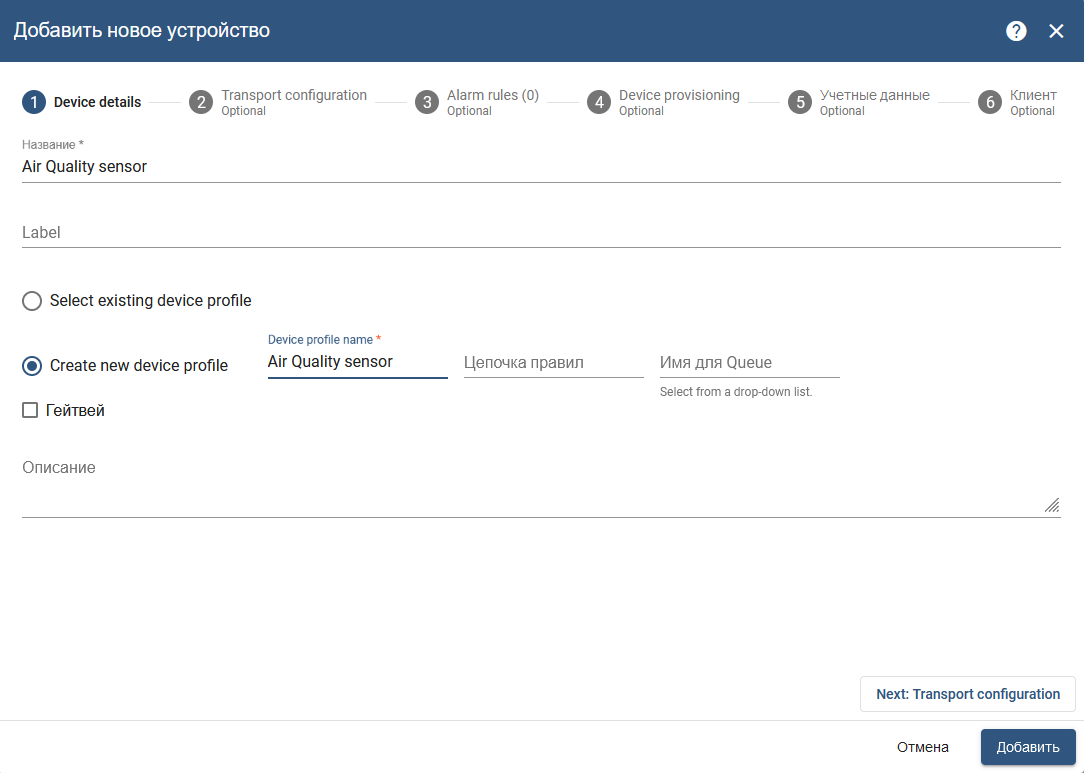
\includegraphics[width=0.7\linewidth]{images/task9-create}
	\caption{Создание устройства на платформе \tb}
	\label{fig:task9-create}
\end{figure}

\begin{figure}[h!]
	\centering
	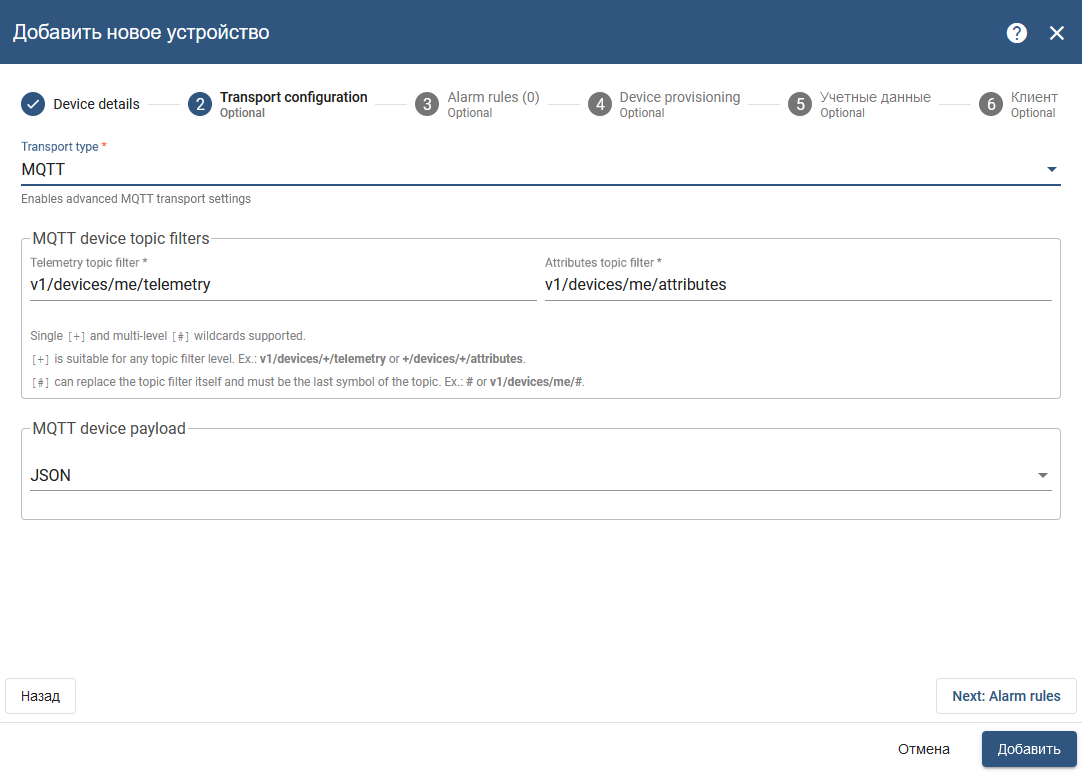
\includegraphics[width=0.7\linewidth]{images/task9-create2}
	\caption{Настройка устройства на платформе \tb}
	\label{fig:task9-create2}
\end{figure}

\subsection{Отправка данных в облако}

Выполним передачу тестовых данных в каждое из созданных устройств, список которых приведен на Рисунке \ref{fig:devices}.

% TODO: \usepackage{graphicx} required
\begin{figure}[h!]
	\centering
	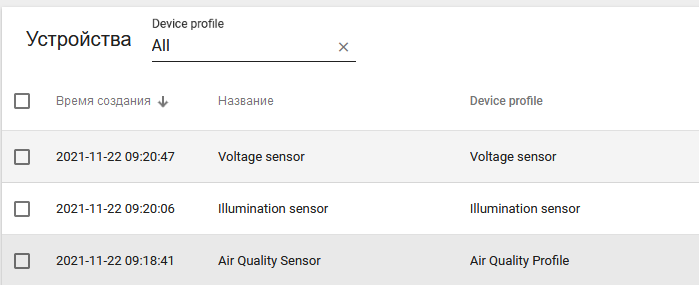
\includegraphics[width=0.66\linewidth]{images/devices}
	\caption{Список зарегистрированных устройств}
	\label{fig:devices}
\end{figure}

Приведем команду, с помощью которой осуществляется процесс ответа на сообщение с телеметрией в топик устройства с параметром "motion" (см. Рисунок (см. Листинг \ref{lst:send}).

\lstinputlisting[caption=Отправка данных на устройство, label=lst:send]{/home/denilai/Documents/repos/latex/scripts/task-9-main.txt}
%
%\begin{figure}[h!]
%	\centering
%	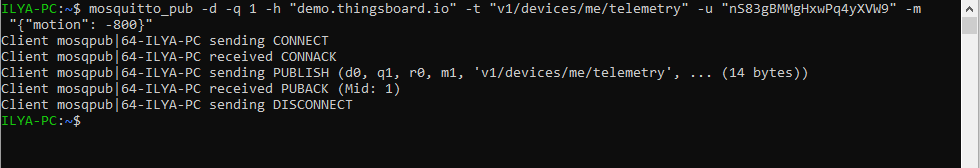
\includegraphics[width=0.7\linewidth]{images/send}
%	\caption{Отправка данных на устройства}
%	\label{fig:send}
%\end{figure}

После отправки, тестовые данные отображаются в веб-интерфейсе платформы \tb в виде представленном на Рисунках \mbox{\ref{fig:voltagedata}--\ref{fig:airqualitydata}}. 
% TODO: \usepackage{graphicx} required
\begin{figure}[h!]
	\centering
	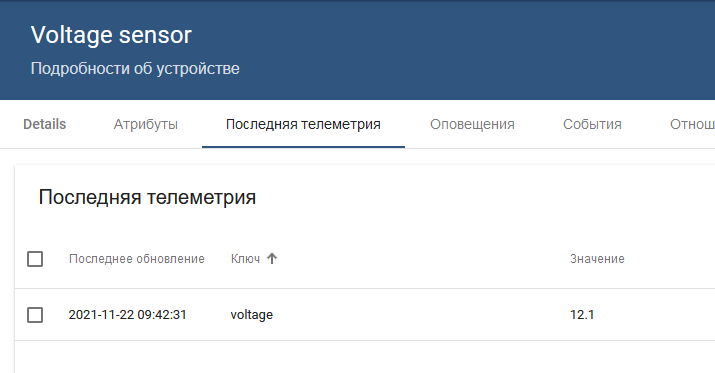
\includegraphics[width=0.7\linewidth]{images/VoltageData}
	\caption{Данные с датчика напряжения}
	\label{fig:voltagedata}
\end{figure}
% TODO: \usepackage{graphicx} required
\begin{figure}[h!]
	\centering
	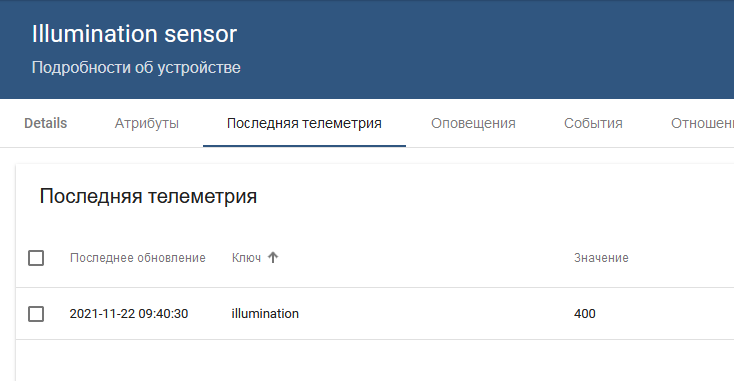
\includegraphics[width=0.7\linewidth]{images/IlluminationData}
	\caption{Данные с датчика освещения}
	\label{fig:illuminationdata}
\end{figure}
% TODO: \usepackage{graphicx} required
\begin{figure}[h!]
	\centering
	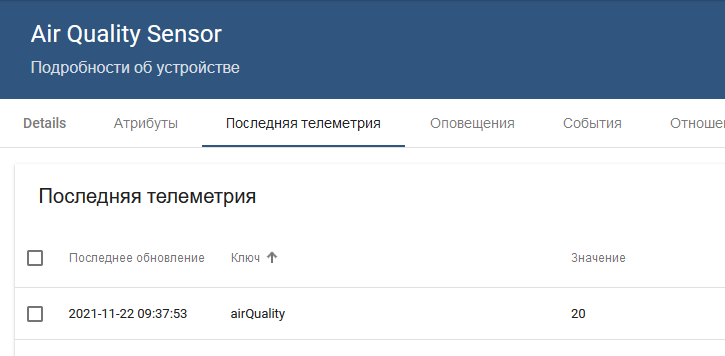
\includegraphics[width=0.7\linewidth]{images/airQualityData}
	\caption{Данные с датчика качества воздуха}
	\label{fig:airqualitydata}
\end{figure}


Данные соответствуют типу устройства и передаются при помощи утилиты \texttt{mosquito\_pub}.

%\newpage

\section{Дополнительное задание №9}
\subsection{Выбор облачного решения}

В качестве облачного решения была выбрана платформа ThingsBoard. Данный выбор был сделан по следующим причинам:
\begin{itemize}
	\item Понятный пользовательский интерфейс;
	\item Популярность платформы;
	\item Возможность установить платформу локально или использовать готовую облачную среду.
\end{itemize}


\subsection{Реализация отправки данных}

Реализуем отправку данных с программного эмулятора реального физического устройства в облачную платформу ThingsBoard. Приведем листинг скрипта на языке программирования Python (см. Листинг \ref{send-to-cloud}):

\lstinputlisting[caption=Отправка данных в облачную платформу, label=send-to-cloud]{\pathToScriptsFolder/dop9-publish.py}

В результате запуска данного скрипта происходит соединение с MQTT-брокером, создание экземпляра класса Client для MQTT-брокера, с последнующей передачей данных в облако (см. Рисунки \ref{fig:dop9-send},  \ref{fig:dop9-recieve}).


% TODO: \usepackage{graphicx} required
\begin{figure}[h!]
	\centering
	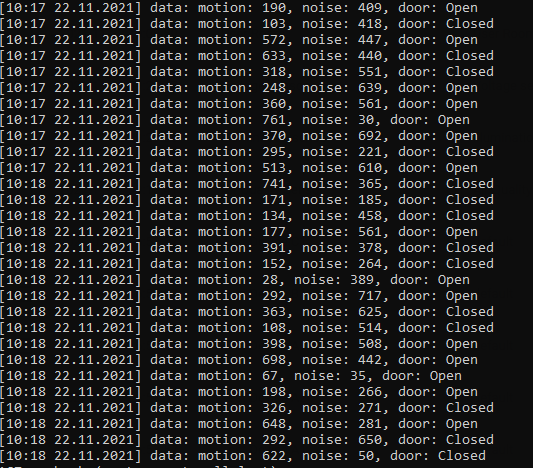
\includegraphics[width=0.6\linewidth]{images/dop9-send}
	\caption{Оправка телеметрических данных с устройств }
	\label{fig:dop9-send}
\end{figure}


% TODO: \usepackage{graphicx} required
\begin{figure}[h!]
	\centering
	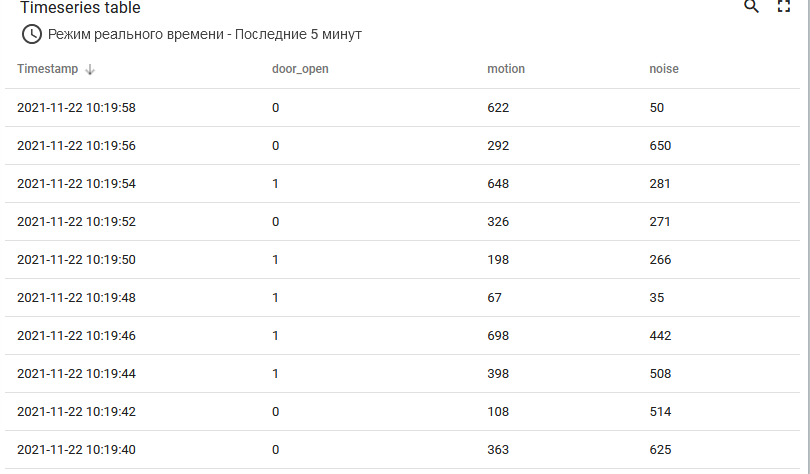
\includegraphics[width=0.6\linewidth]{images/dop9-recieve}
	\caption{Прием телеметрических данных облачной платформой}
	\label{fig:dop9-recieve}
\end{figure}
%\hfill\newpage\hfill\newpage
\newpage
\section{Практическая работа №10}

Реализуем следующие сценарии из практической работы №3 при помощи цепочек правил ThingsBoard.

\begin{enumerate}
	\item Включение и выключение вентилятора по датчику движения;
	\item Включение и выключения индикации зеленым и красным светом комбинированного датчика по кнопкам.
\end{enumerate}

\subsection{Реализация сценария управления вентилятором}
На платформе \tb создадим виртуальное устройство, которое будет прообразом реального вентилятора (см. Рисунок \ref{fig:dev}).

% TODO: \usepackage{graphicx} required
\begin{figure}[h!]
	\centering
	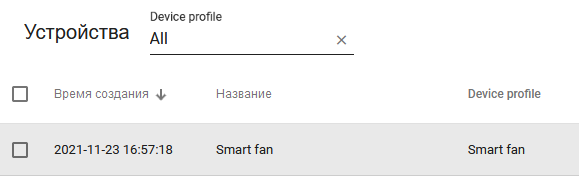
\includegraphics[width=0.6\linewidth]{images/dev}
	\caption{Виртуальный вентилятор}
	\label{fig:dev}
\end{figure}

Создадим цепочку правил для контроля за состоянием вентилятора. Когда значения, передаваемые датчиком движения превышают 700 условных единиц, вентилятор должен включаться. При уменьшении значения ниже 700, вентилятор должен выключаться. Приведенная на Рисунке \ref{fig:chains} цепочка правил описывает данный сценарий управления устройством.

% TODO: \usepackage{graphicx} required
\begin{figure}[h!]
	\centering
	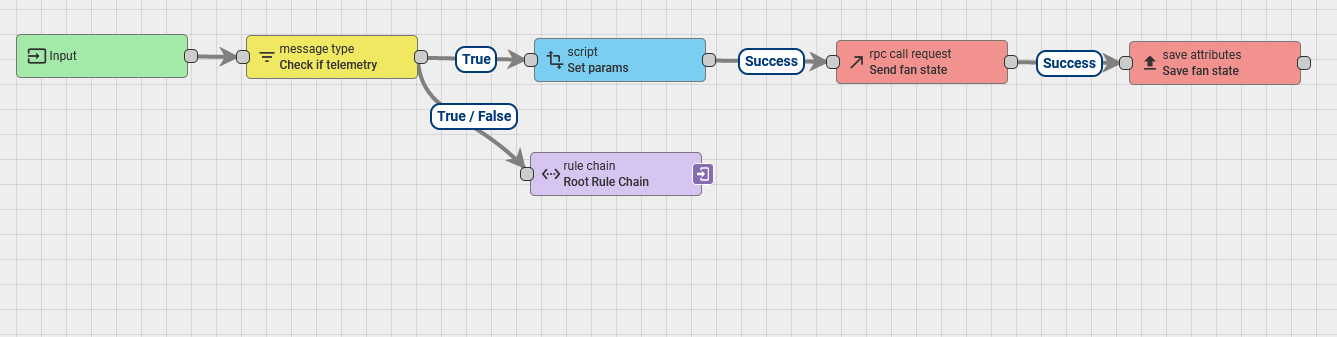
\includegraphics[width=0.6\linewidth]{images/chains}
	\caption{Цепочка правил для управления вентилятором}
	\label{fig:chains}
\end{figure}


\textbf{Узел формирования параметров вентилятора}

Узел трансформации данных при помощи скрипта позволяет переформировать объект,
содержащий в себе данные приходящего сообщения: его основную полезную нагрузку,
метаданные, а также тип сообщения.

Поведение узла описывается при помощи Java Script. Изначально в приходящей телеметрии
предполагается наличие параметра \texttt{motion}. На основании этого параметра
вычисляет новое состояние увлажнителя и формируется новый объект сообщения с этим
состоянием. 

Данный объект содержит в себе несколько свойств: \textit{method} --- это наименование
метода, при помощи которого можно будет идентифицировать необходимое действие на
устройстве, а также свойство \textit{params}, содержащее как раз состояние устройства, в которое
его необходимо привести. 

В дальнейшем этот объект будет отправлен на конечное
устройство для смены его состояния. Изменим тип события на событие загрузки
атрибутов устройства --- POST\_ATTRUBUTE\_REQUEST. Узел возвращает объект, содержащий в себе основное
сообщение, метаданные, а также тип сообщения. Полный код приведен в Листинге \ref{send-to-object}.


\lstinputlisting[caption=Отправка объекта на устройство, label=send-to-object]{\pathToScriptsFolder/fan_chain.js}

После реализации узла формирования параметров можно приступать к тестированию созданной цепочки. 

Подпишемся на топик запросов (v1/devices/me/rpc/request/+) созданного для данного
виртуального вентилятора. Воспользуемся для этого следующую командой:
%\newpage
\begin{lstlisting}
	mosquitto_sub -v -h "demo.thingsboard.io" -t "v1/devices/me/rpc/request/+" -u "nS83gBMMgHxwPq4yXVW9"
\end{lstlisting}

После чего опубликуем сообщение с телеметрией в топик устройства с параметром
\texttt{motion}:

\begin{lstlisting}
mosquitto_pub -d -q 1 -h "demo.thingsboard.io" -t "v1/devices/me/telemetry" -u "nS83gBMMgHxwPq4yXVW9" -m "{"motion": 800}"
\end{lstlisting}

% TODO: \usepackage{graphicx} required
\begin{figure}[h!]
	\centering
	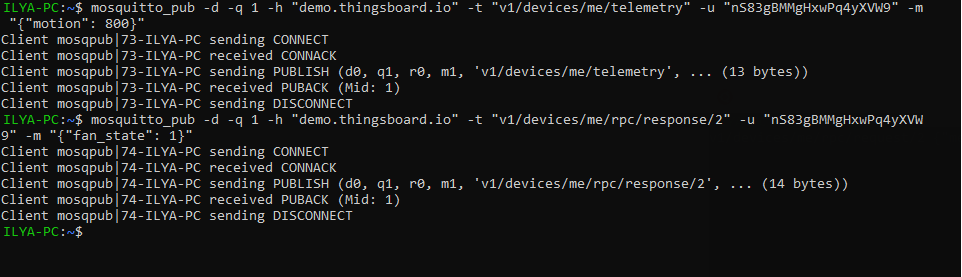
\includegraphics[width=0.6\linewidth]{images/t1-sender}
	\caption{Публикация сообщения с телеметрией вентилятора}
	\label{fig:t1-sender}
\end{figure}

Чтобы отправить ответ на опубликованный запрос на смену состояния, воспользуемся
также утилитой \texttt{mosquito\_pub}.

Для отправки ответа на созданный запрос необходимо послать сообщение в топик
\textit{v1/devices/me/rpc/response/<request-id>}. Воспользуемся для этого следующей командой:

\begin{lstlisting}
	mosquitto_pub -d -q 1 -h "demo.thingsboard.io" -t "v1/devices/me/rpc/response/2" -u "nS83gBMMgHxwPq4yXVW9" -m "{"fan_state": 1}"
\end{lstlisting}

После этого можно проверить в облаке поступившую телеметрию и аргументы устройства,
посланные в ответ на запрос. Результаты представлены на Рисунках \ref{fig:tel} и \ref{fig:attr}.

% TODO: \usepackage{graphicx} required
\begin{figure}[h!]
	\centering
	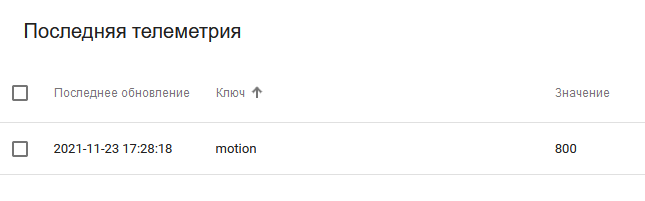
\includegraphics[width=0.6\linewidth]{images/tel}
	\caption{Телеметрия облачного устройства <<вентилятор>>}
	\label{fig:tel}
\end{figure}


\begin{figure}[h!]
	\centering
	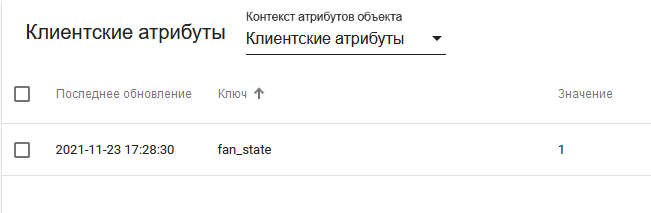
\includegraphics[width=0.6\linewidth]{images/attr}
	\caption{Атрибуты облачного устройства <<вентилятор>>}
	\label{fig:attr}
\end{figure}


\subsection{Реализация сценария управления лампами}


На платформе \tb создадим виртуальное устройство, которое будет прообразом реальных блока светодиодных ламп (см. Рисунок \ref{fig:dev-2}).


% TODO: \usepackage{graphicx} required
\begin{figure}[h!]
	\centering
	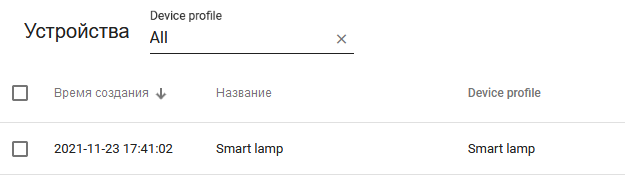
\includegraphics[width=0.5\linewidth]{images/dev-2}
	\caption{Виртуальный блок ламп}
	\label{fig:dev-2}
\end{figure}


Создадим цепочку правил для контроля за состоянием блока ламп. Световые индикаторы должны сигнализировать о включении и выключении комбинированного датчика. При включении датчика следует включить зеленую лампу, а при выключении --- красную. 

Приведенная на Рисунке \ref{fig:chains-2} цепочка правил описывает данный сценарий управления устройством.
% TODO: \usepackage{graphicx} required
\begin{figure}[h!]
	\centering
	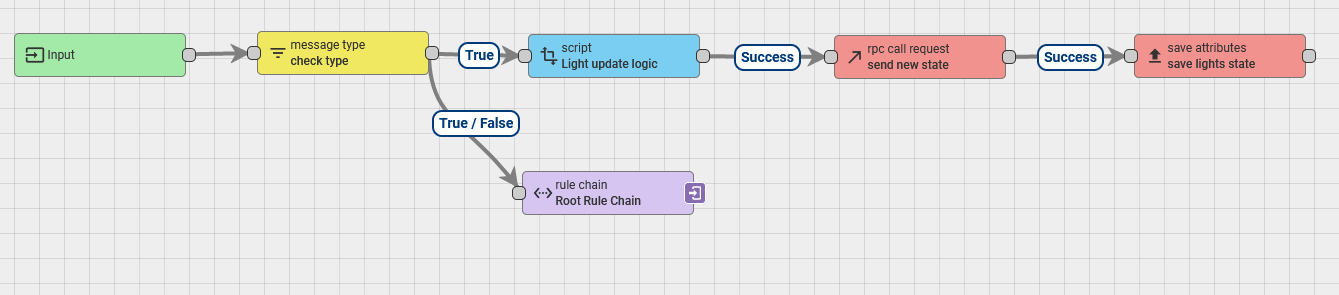
\includegraphics[width=0.6\linewidth]{images/chains-2}
	\caption{Цепочка правил для управления блоком ламп}
	\label{fig:chains-2}
\end{figure}


\textbf{Узел формирования параметров вентилятора}

Полный код, описывающий поведение узла формирования параметров блока умных ламп приведен в Листинге \ref{lamp}.


\lstinputlisting[caption=Блок умных ламп, label=lamp]{\pathToScriptsFolder/light_chain.js}

После реализации узла формирования параметров можно приступать к тестированию созданной цепочки. 

Подпишемся на топик запросов (v1/devices/me/rpc/request/+) созданного для данного
виртуального контроллера. Воспользуемся для этого следующую командой:

\begin{lstlisting}
mosquitto_sub -v -h "demo.thingsboard.io" -t "v1/devices/me/rpc/request/+" -u "RxcWZHP60DTvKzcgWB0T"
\end{lstlisting}

После чего опубликуем сообщение с телеметрией в топик устройства с параметрами
\texttt{redButton} и \texttt{greenButton}:

\begin{lstlisting}
mosquitto_pub -d -q 1 -h "demo.thingsboard.io" -t "v1/devices/me/telemetry" -u "RxcWZHP60DTvKzcgWB0T" -m "{"redButton": 1, "greenButton": 0}"
\end{lstlisting}

% TODO: \usepackage{graphicx} required
\begin{figure}[h!]
	\centering
	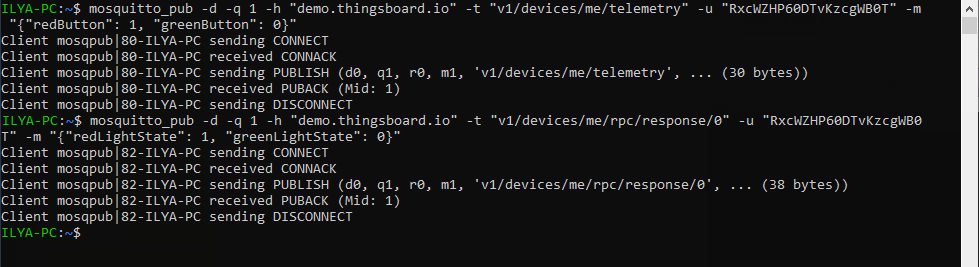
\includegraphics[width=0.6\linewidth]{images/t2-sender}
	\caption{Публикация сообщения с телеметрией блока ламп}
	\label{fig:t2-sender}
\end{figure}

Чтобы отправить ответ на опубликованный запрос на смену состояния, воспользуемся
также утилитой \texttt{mosquito\_pub}.

Для отправки ответа на созданный запрос необходимо послать сообщение в топик
\textit{v1/devices/me/rpc/response/<request-id>}. Воспользуемся для этого следующей командой:

\begin{lstlisting}
mosquitto_pub -d -q 1 -h "demo.thingsboard.io" -t "v1/devices/me/rpc/response/2" -u "RxcWZHP60DTvKzcgWB0T" -m "{"redLightState": 1, "greenLightState": 0}"
\end{lstlisting}

После этого можно проверить в облаке поступившую телеметрию и аргументы устройства,
посланные в ответ на запрос. Результаты представлены на Рисунках \ref{fig:tel-2} и \ref{fig:attr-2}.

% TODO: \usepackage{graphicx} required
\begin{figure}[h!]
	\centering
	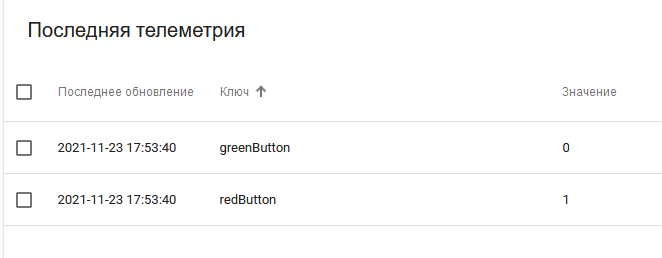
\includegraphics[width=0.6\linewidth]{images/tel-2}
	\caption{Телеметрия облачного устройства <<блок светодиодных ламп>>}
	\label{fig:tel-2}
\end{figure}


\begin{figure}[h!]
	\centering
	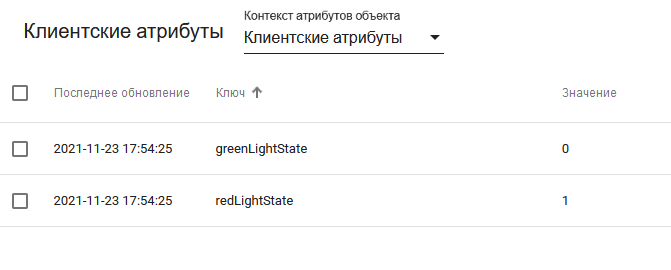
\includegraphics[width=0.6\linewidth]{images/attr-2}
	\caption{Атрибуты облачного устройства <<блок светодиодных ламп>>}
	\label{fig:attr-2}
\end{figure}


\section{Дополнительное задание № 10}

\subsection{Описание взаимодействия пользователя с интерфейсом}
Опишем взаимодействие пользователя с интерфейсом реализуемой системы при помощи диаграммы Use-case в нотации UML (см. Рисунок \ref{fig:usecase-10}). 

% TODO: \usepackage{graphicx} required
\begin{figure}[h!]
	\centering
	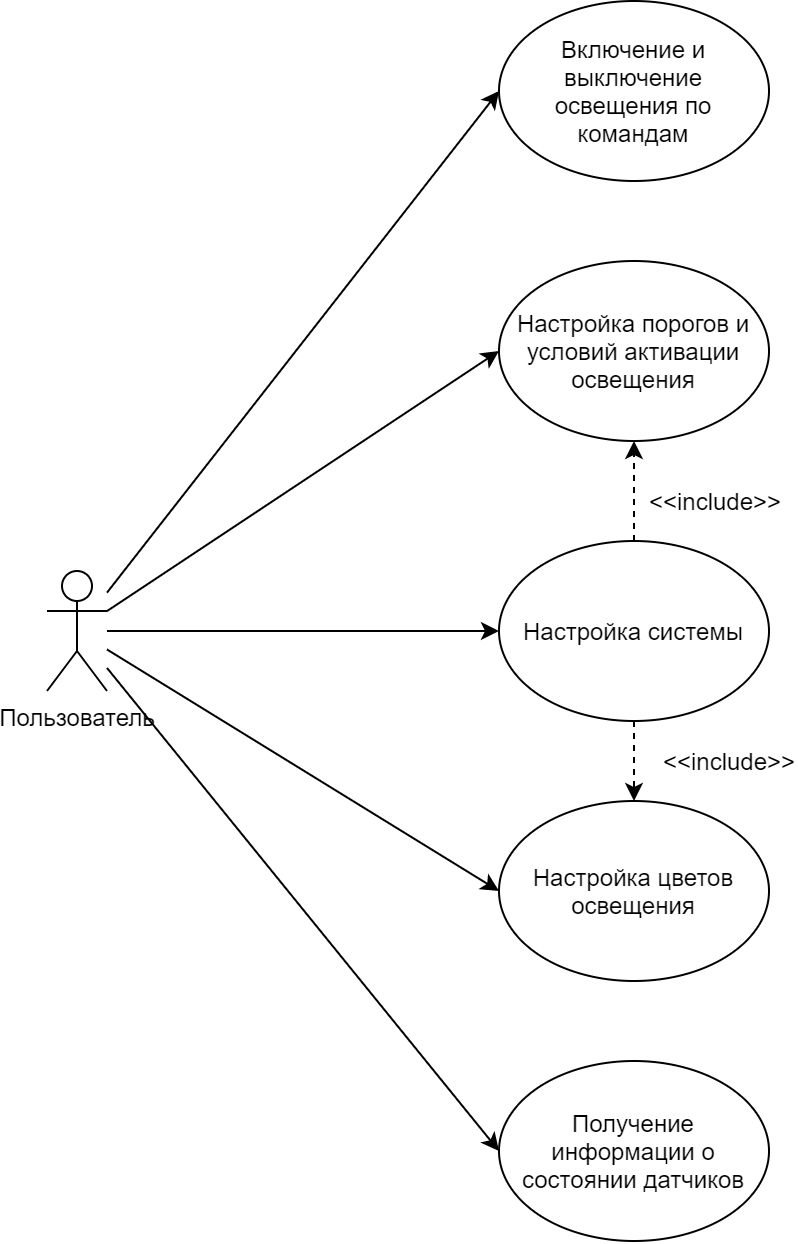
\includegraphics[width=0.4\linewidth]{images/usecase-10}
	\caption{Взаимодействие пользователя с системой}
	\label{fig:usecase-10}
\end{figure}


\subsection{Требования к интерфейсу пользователя}

Для разрабатываемого нами программного решения был выбран интерфейс \mbox{Telegram--бота}. Взаимодействие с данным интерфейсом состоит в отправке текстовых сообщений в мессенджере и основано на принципе <<запрос--ответ>> --- данные предоставляются пользователю по требованию.

Для удобного взаимодействия с информационной системой данные должны предоставляться пользователю в графическом, табличном и текстовом виде. Это упросит взаимодействие с программным инструментом.


Следует реализовать возможность выбора отслеживаемого на данный момент датчика, регистрации нового датчика (прибора), получения сведений о состоянии измерительного прибора, получении текущей телеметрии и статистических данных.

Сведения о передаваемой датчиками телеметрии следует представлять в виде таблиц, графиков или структурированного текста. Также нужно предоставить пользователю возможность получать сведения о данных за определенный временной промежуток, проводить их агрегирование.



\subsection{Макеты интерфейса приложения}

После проведения анализа существующих решений было сформировано представление о том, как следует выстроить взаимодействие с пользователем. 

Пользователю предлагается набор команд, которые понимает \mbox{Telegram--бот}, их список приведен над полем ввода. На каждую команду бот отвечает установленным образом, предоставляя пользователю информацию о состоянии элементов системы. 

Решения, использующие аналогичный интерфейс взаимодействия приведены на Рисунках \mbox{\ref{fig:drewb}--\ref{fig:wash}}.


% TODO: \usepackage{graphicx} required
\begin{figure}[h!]
	\centering
	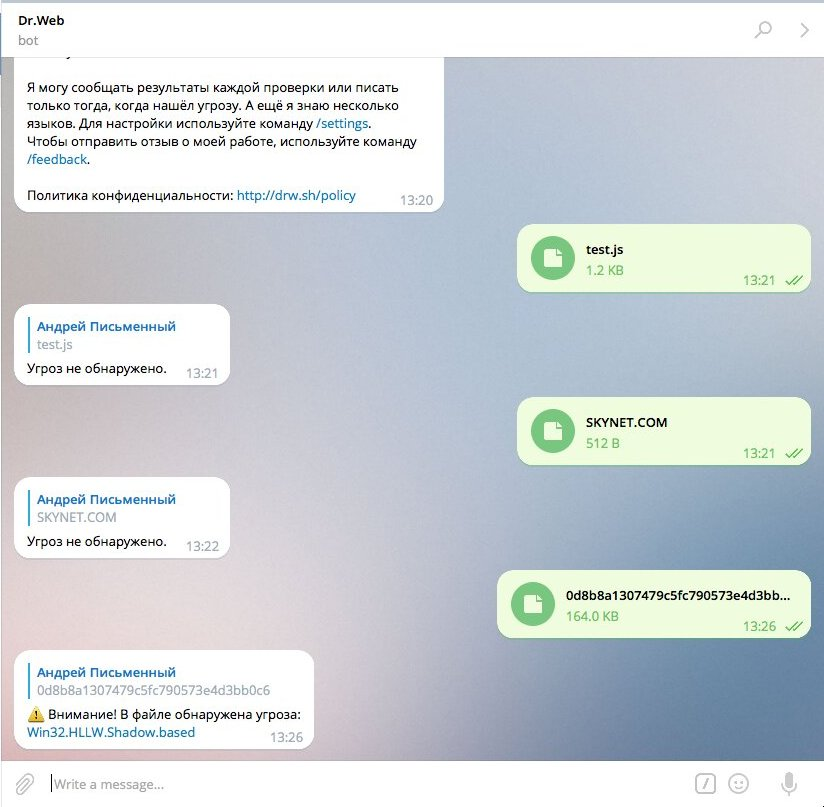
\includegraphics[width=0.5\linewidth]{images/mokups/drewb}
	\caption{Макет 1}
	\label{fig:drewb}
\end{figure}

\begin{figure}[h!]
	\centering
	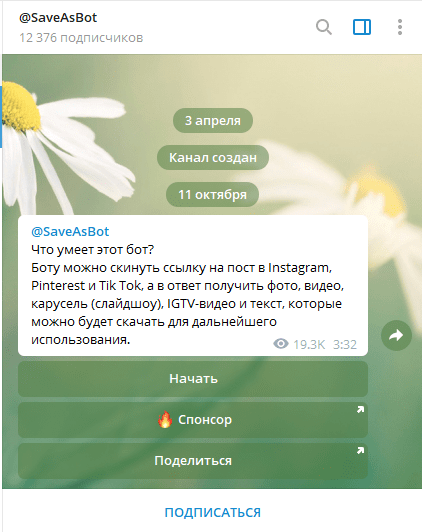
\includegraphics[width=0.5\linewidth]{images/mokups/saver}
	\caption{Макет 2}
	\label{fig:saver}
\end{figure}

% TODO: \usepackage{graphicx} required
\begin{figure}[h!]
	\centering
	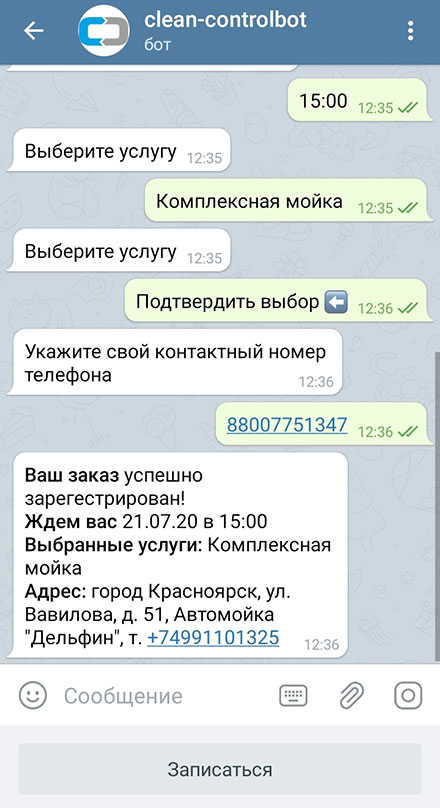
\includegraphics[width=0.4\linewidth]{images/mokups/wash}
	\caption{Макет 3}
	\label{fig:wash}
\end{figure}
% TODO: \usepackage{graphicx} required
\clearpage

\section{Практическая работа № 11}

%\subsection{Добавление обработчиков тревожных сигналов}
\subsection{Обработка тревожных сигналов вентилятора}

Добавим в цепочки правил управления вентилятором тревогу при выходе приходящего параметра за допустимые границы, а также тревогу при поступлении неверного ответа от физического устройства.

Для реализации механизма тревог внесем изменения в цепочку правил для управления умным вентилятором~---~добавим узел сохранения атрибутов запроса \textit{(Save request atributes)} перед узлом отправки запроса и узел получения атрибутов запроса \textit{(Get request atributes)} вместо последнего узла сохранения атрибутов ответа.

Также добавим два узла проверки атрибутов и статуса возвращаемого от устройства ответа \textit{(Check request answer)}. Осуществим проверку при помощи двух скриптов из раздела фильтрующих блоков.
Приведем скрипты проверки параметров (см. Листинги \ref{filter-1.1}, \ref{filter-1.2}):

\lstinputlisting[caption=Проверка абсолютных значений приходящего параметра, label=filter-1.1]{\pathToScriptsFolder/rule-chain-filter-1.js}


\lstinputlisting[caption=Проверка корректности значений приходящего параметра, label=filter-1.2]{\pathToScriptsFolder/rule-chain-filter-2.js}


Поскольку параметры для запроса были записаны в JSON формате необходимо распарсить JSON строку в объект JS для извлечения параметров при помощи функции JSON.parse. 
Подключим получившийся узел к узлу получения атрибутов запроса.

Далее создадим два узла активации тревоги в случае, если проверка не будет пройдена. Создадим узел \textit{Create alarm}, отвечающий за проверку соответствия параметров заданному диапазону и зададим ему следующий скрипт в качестве обработчика (см. Листинг \ref{alarm-1.3}).

\newpage

\lstinputlisting[caption=Формирование тревоги в случае выхода значений параметра за установленные границы, label=alarm-1.3]{\pathToScriptsFolder/rule-chain-alarm-1.js}

Создадим узел \textit{Create alarm}, отвечающий за проверку корректности параметров и зададим ему следующий скрипт в качестве обработчика (см. Листинг \ref{alarm-1.4}).

\lstinputlisting[caption=Формирование тревоги по случаю некорректности приходящих параметров, label=alarm-1.4]{\pathToScriptsFolder/rule-chain-alarm-2.js}


Приведем измененную цепочку правил (см. Рисунок \ref{fig:chain-fan}).
\begin{figure}[h!]
	\begin{minipage}[h!]{\linewidth}
		\center{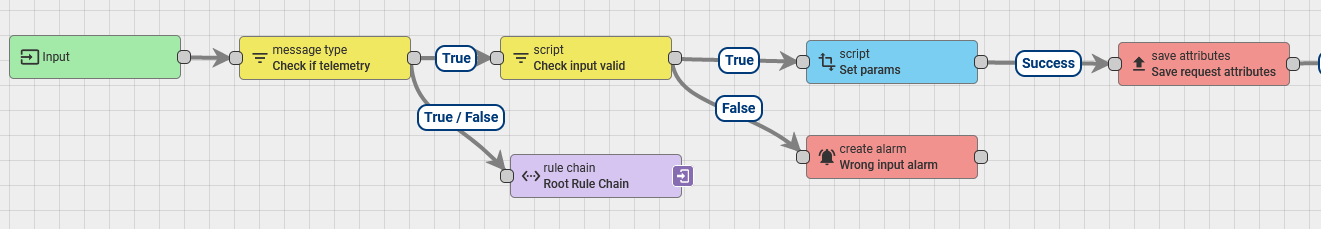
\includegraphics[width=\linewidth]{rule-chain-1}\\ а)}
	\end{minipage}

	\begin{minipage}[h!]{\linewidth}
		\center{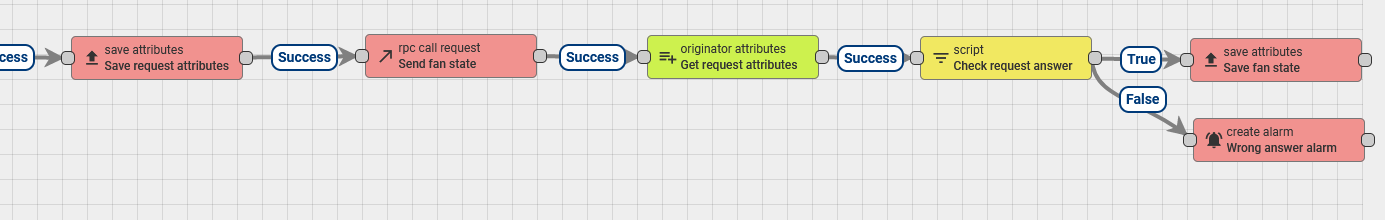
\includegraphics[width=\linewidth]{rule-chain-2}\\ б)}
	\end{minipage}
	\captionof{figure}{Измененная цепочка управления умным вентилятором}
	\label{fig:chain-fan}
\end{figure}
\newpage
\subsection*{Тестирование цепочки правил}
\label{sec:fan-test}
Проведем тестирование созданной цепочки при помощи утилит mosquitto.

Подпишемся на топики виртуального устройства (см Рисунок \ref{fig:t1-sub}).
% TODO: \usepackage{graphicx} required
\begin{figure}[h!]
	\centering
	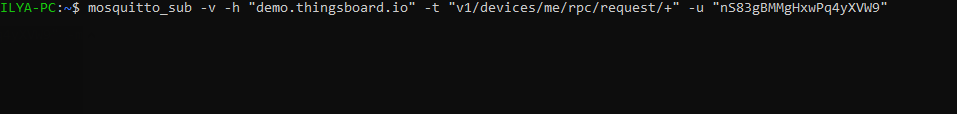
\includegraphics[width=1\linewidth]{images/t1-sub}
	\caption{Подписка на топик умного вентилятора}
	\label{fig:t1-sub}
\end{figure}

Протестируем цепочку при отправке параметром, выходящих за границы определенного диапазона (см. Рисунок \ref{fig:t1-pub-range}).

% TODO: \usepackage{graphicx} required
\begin{figure}[h!]
	\centering
	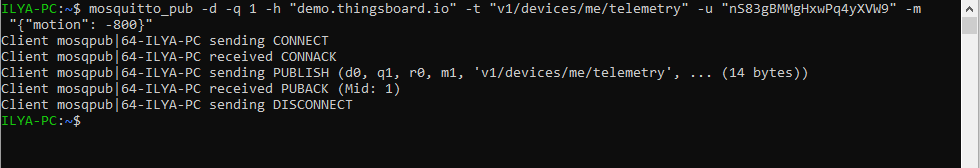
\includegraphics[width=1\linewidth]{images/t1-pub-range}
	\caption{Отправка некорректной телеметрии}
	\label{fig:t1-pub-range}
\end{figure}

Вслед за эти ThingsBoard отправит оповещение уровня \textit{Critital} (см. Рисунок \ref{fig:alarm-input-value}).

% TODO: \usepackage{graphicx} required
\begin{figure}[h!]
	\centering
	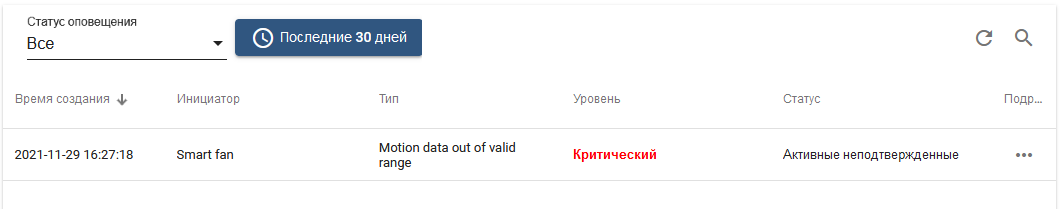
\includegraphics[width=1\linewidth]{images/alarm-input-value}
	\caption{Тревога. Данные выходят за границы заданного диапазона}
	\label{fig:alarm-input-value}
\end{figure}

Приведем подробные сведения о тревоге (см. Рисунок \ref{fig:alarm-input-value-detail}).


% TODO: \usepackage{graphicx} required
\begin{figure}[h!]
	\centering
	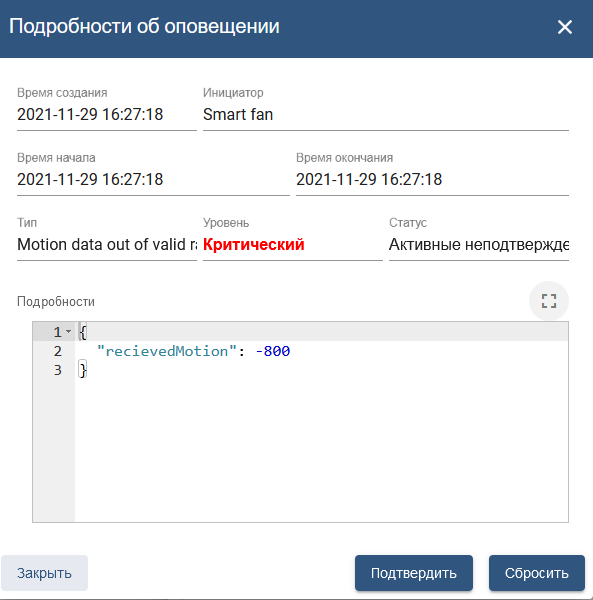
\includegraphics[width=0.7\linewidth]{images/alarm-input-value-detail}
	\caption{Подробные сведения о тревоге}
	\label{fig:alarm-input-value-detail}
\end{figure}

\newpage
Протестируем цепочку при получении неверного ответа от устройства. Отправим данные об уровне движения в диапазоне, в котором должно происходить включение вентилятора. Вместе с этим отправим сообщение о выключении вентилятора, что противоречит ожидаемому поведению прибора (см. Рисунок \ref{fig:listen-p2}).

% TODO: \usepackage{graphicx} required
\begin{figure}[h!]
	\centering
	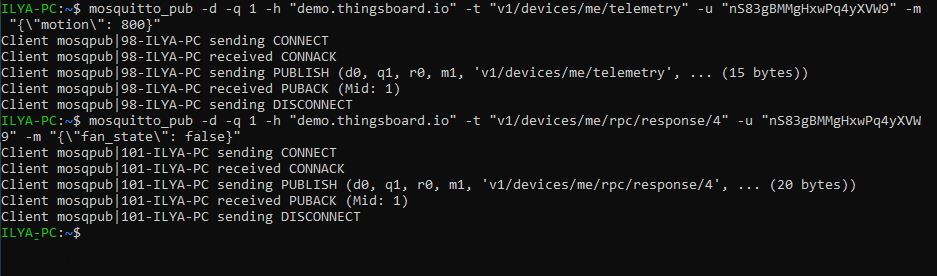
\includegraphics[width=1\linewidth]{images/listen-p2}
	\caption{Запись некорректных данных в топик}
	\label{fig:listen-p2}
\end{figure}

% TODO: \usepackage{graphicx} required
\begin{figure}[h!]
	\centering
	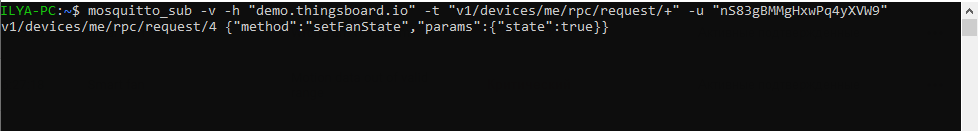
\includegraphics[width=1\linewidth]{../../../../../Москва/IoT/11-osn/send-p2}
	\caption{Подписка на топик умного вентилятора}
	\label{fig:send-p2}
\end{figure}


Платформа ThingsBoard уведомит о некорректности отправленного сообщения, сравнив его с ожидаемым результатом и сгенерирует соответствующий тревожный сигнал (см. Рисунок \ref{fig:alarm-wrong-response}).

% TODO: \usepackage{graphicx} required
\begin{figure}[h!]
	\centering
	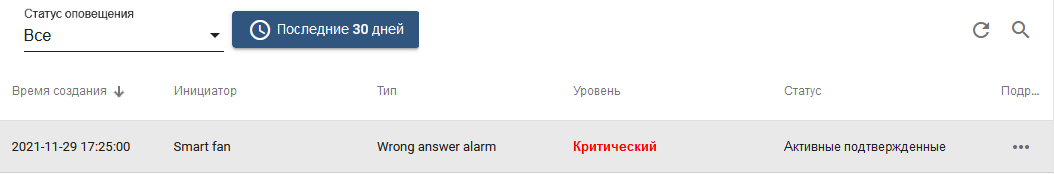
\includegraphics[width=1\linewidth]{images/alarm-wrong-response}
	\caption{Тревога. Некорректные данные}
	\label{fig:alarm-wrong-response}
\end{figure}
\newpage
Приведем подробности тревоги (см. Рисунок \ref{fig:alarm-wrong-response-detail}).
% TODO: \usepackage{graphicx} required
\begin{figure}[h!]
	\centering
	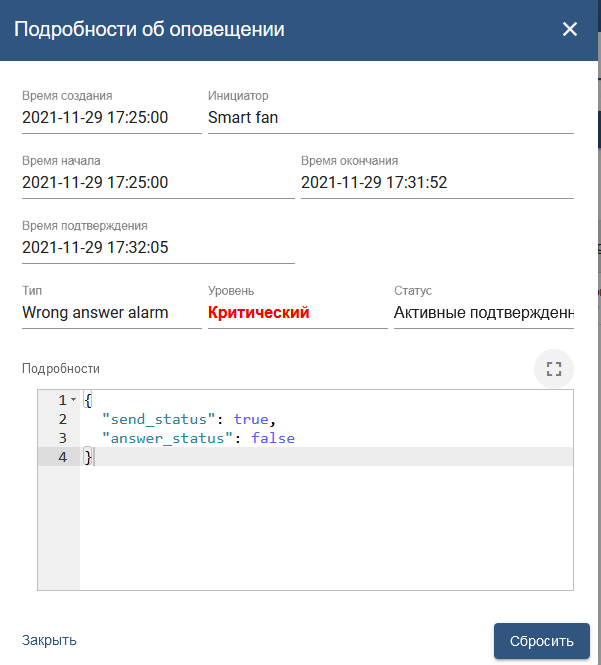
\includegraphics[width=0.6\linewidth]{images/alarm-wrong-response-detail}
	\caption{Подробные сведения о тревоге}
	\label{fig:alarm-wrong-response-detail}
\end{figure}

Сымитировав оба сценария, мы убедились в том, что цепочка правил управления умным вентилятором отработала корректно. Тревоги сработали в соответствии с установленными правилами.
%\newpage

\subsection{Обработка тревожных сигналов блока ламп}

Для цепочки управления блоком ламп добавим тревогу при отсутствии ожидаемого параметра в приходящем сообщении, а также тревогу при поступлении неверного ответа от физического устройства.

Проделаем аналогичные шаги. Создадим узел проверки атрибутов и статуса возвращаемого от устройства ответа \textit{(Check request answer)}, отвечающий за проверку наличия необходимых параметров (см. Листинг \ref{filter-2.1}).

\lstinputlisting[caption=Проверка наличия требуемых параметров, label=filter-2.1]{\pathToScriptsFolder/t2-rule-chain-filter-1.js}

Создадим узел проверки атрибутов и статуса возвращаемого от устройства ответа \textit{(Check request answer)}, отвечающий за проверку корректности приходящих параметров (см. Листинг \ref{filter-2.2}).
%\newpage

\lstinputlisting[caption=Проверка корректности значений приходящего параметра, label=filter-2.2]{\pathToScriptsFolder/t2-rule-chain-filter-2.js}



Поскольку параметры для запроса были записаны в JSON формате необходимо распарсить JSON строку в объект JS для извлечения параметров при помощи функции JSON.parse. 
Подключим получившийся узел к узлу получения атрибутов запроса.

Далее создадим узел активации тревоги в случае, если проверка не будет пройдена. Создадим узел \textit{Create alarm}, инициирующий тревогу в случае отсутствия необходимых параметров и зададим ему следующий скрипт в качестве обработчика (см. Листинг \ref{alarm-2.3}).

\lstinputlisting[caption=Формирование тревоги в случае отсутствия необходимых, label=alarm-2.3]{\pathToScriptsFolder/t2-rule-chain-alarm-1.js}

Создадим узел \textit{Create alarm}, отвечающий за проверку корректности параметров и зададим ему следующий скрипт в качестве обработчика (см. Листинг \ref{alarm-2.4}).

\lstinputlisting[caption=Формирование тревоги по случаю некорректности приходящих параметров, label=alarm-2.4]{\pathToScriptsFolder/t2-rule-chain-alarm-2.js}


Приведем измененную цепочку правил (см. Рисунок \ref{fig:chain-lamp}).
\begin{figure}[h!]
	\begin{minipage}[h!]{\linewidth}
		\center{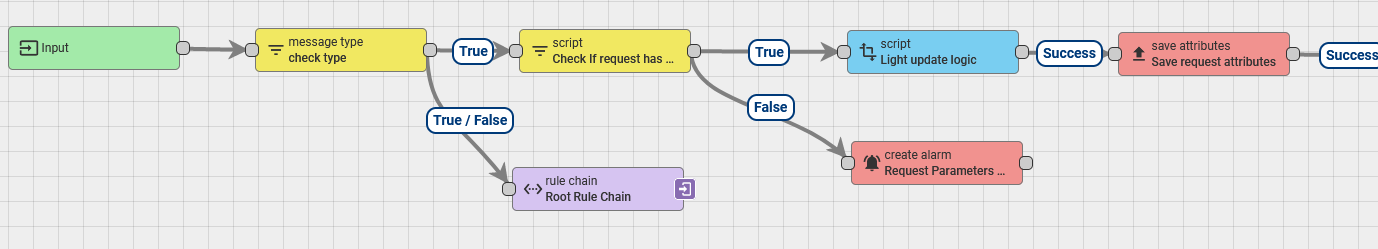
\includegraphics[width=\linewidth]{t2-rule-chain-1}\\ а)}
	\end{minipage}
	
	\begin{minipage}[h!]{\linewidth}
		\center{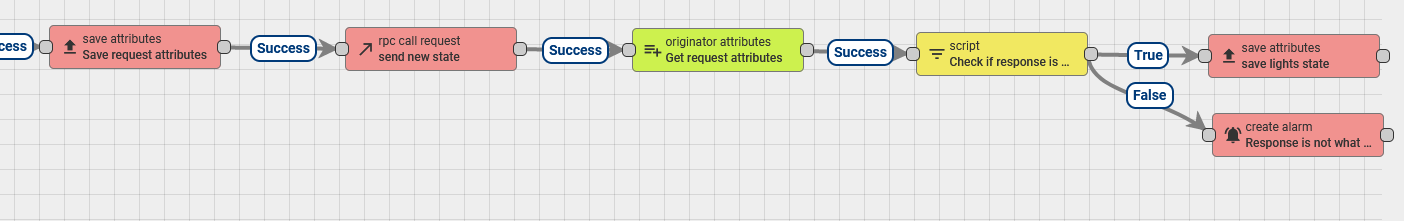
\includegraphics[width=\linewidth]{t2-rule-chain-2}\\ б)}
	\end{minipage}
	\captionof{figure}{Измененная цепочка управления блоком умных ламп}
	\label{fig:chain-lamp}
\end{figure}

\subsection*{Тестирование цепочки правил}
\label{sec:lamp-test}

Проведем тестирование созданной цепочки при помощи утилит mosquitto.

Подпишемся на топики виртуального устройства (см Рисунок \ref{fig:t2-listen-p2}).
% TODO: \usepackage{graphicx} required
\begin{figure}[h!]
	\centering
	\includegraphics[width=1\linewidth]{images/t2-listen-p2}
	\caption{Подписка на топик блока умных ламп}
	\label{fig:t2-listen-p2}
\end{figure}

Протестируем цепочку при отправке сообщения с неверным количеством параметров (см. Рисунок \ref{fig:t2-send}).

% TODO: \usepackage{graphicx} required
\begin{figure}[h!]
	\centering
	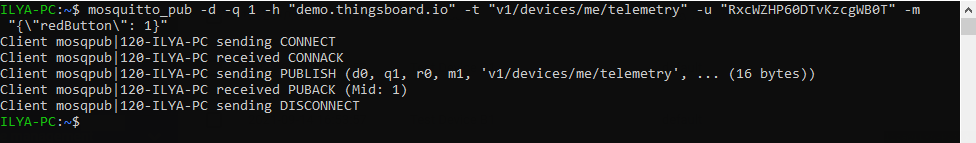
\includegraphics[width=1\linewidth]{images/t2-send}
	\caption{Отправка телеметрии с отсутствующими параметрами}
	\label{fig:t2-send}
\end{figure}

Вслед за эти ThingsBoard отправит оповещение уровня \textit{Critital} (см. Рисунок \ref{fig:t2-alarm-missing-params}).

% TODO: \usepackage{graphicx} required
\begin{figure}[h!]
	\centering
	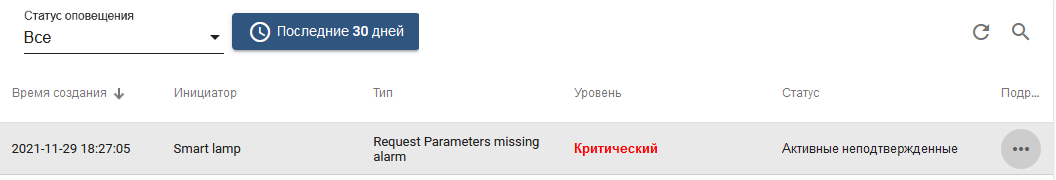
\includegraphics[width=1\linewidth]{images/t2-alarm-missing-params}
	\caption{Тревога. Необходимый параметр отсутствует}
	\label{fig:t2-alarm-missing-params}
\end{figure}

Приведем подробные сведения о тревоге (см. Рисунок \ref{fig:t2-alarm-missing-params-detail}).


% TODO: \usepackage{graphicx} required
\begin{figure}[h!]
	\centering
	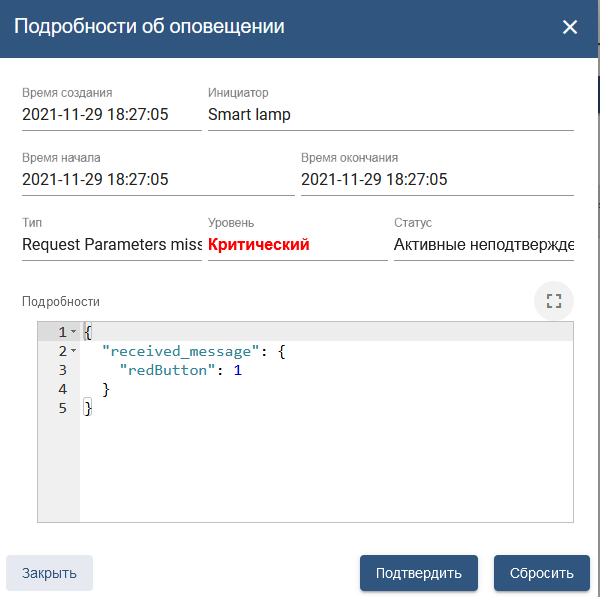
\includegraphics[width=0.7\linewidth]{images/t2-alarm-missing-params-detail}
	\caption{Подробные сведения о тревоге}
	\label{fig:t2-alarm-missing-params-detail}
\end{figure}

Протестируем цепочку при получении неверного ответа от устройства. Отправим данные об уровне движения в диапазоне, в котором должно происходить включение вентилятора. Вместе с этим отправим сообщение о выключении вентилятора, что противоречит ожидаемому поведению прибора. (см. Рисунок \ref{fig:t2-send-p2}).

% TODO: \usepackage{graphicx} required
\begin{figure}[h!]
	\centering
	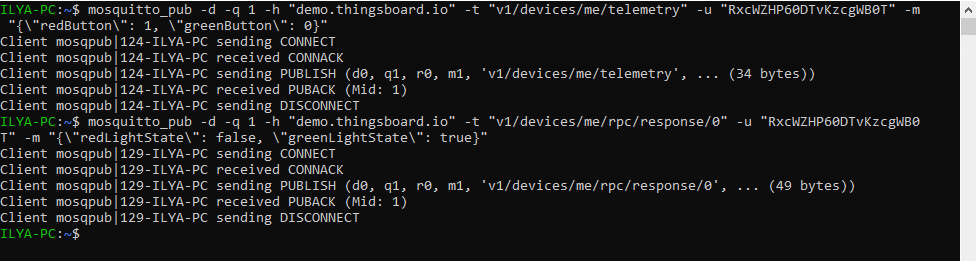
\includegraphics[width=1\linewidth]{images/t2-send-p2}
	\caption{Отправка некорректных данных}
	\label{fig:t2-send-p2}
\end{figure}
% TODO: \usepackage{graphicx} required
\begin{figure}[h!]
	\centering
	\includegraphics[width=1\linewidth]{../../../../../Москва/IoT/11-osn/t2-listen-p2}
	\caption{Подписка на топик блока умных ламп}
	\label{fig:t2-listen-p2w}
\end{figure}

Платформа ThingsBoard уведомит о некорректности отправленного сообщения, сравнив его с ожидаемым результатом и cгенерирует соответствующий тревожный сигнал (см. Рисунок \ref{fig:t2-alarm-wrong-response}).

% TODO: \usepackage{graphicx} required
\begin{figure}[h!]
	\centering
	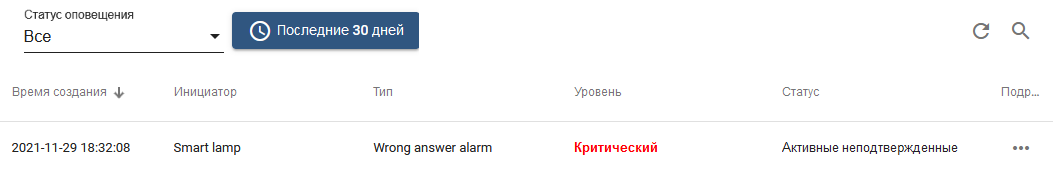
\includegraphics[width=1\linewidth]{images/t2-alarm-wrong-response}
	\caption{Тревога. Некорректные данные}
	\label{fig:t2-alarm-wrong-response}
\end{figure}

Приведем подробности тревоги (см. Рисунок \ref{fig:t2-alarm-wrong-response-detail}).
% TODO: \usepackage{graphicx} required
\begin{figure}[h!]
	\centering
	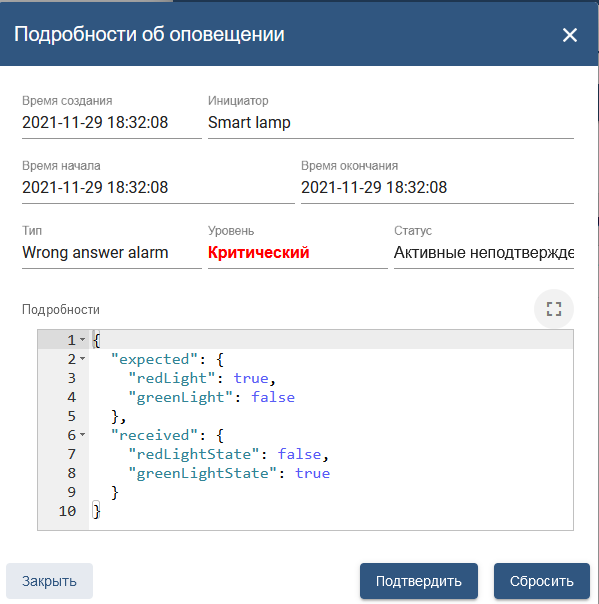
\includegraphics[width=0.7\linewidth]{images/t2-alarm-wrong-response-detail}
	\caption{Подробные сведения о тревоге}
	\label{fig:t2-alarm-wrong-response-detail}
\end{figure}

Сымитировав оба сценария, мы убедились в том, что цепочка правил управления блоком умных ламп отработала корректно. Тревоги сработали в соответствии с установленными правилами.

\section{Дополнительное задание № 11}

\subsection{Описание технологического стека проекта}

Пользовательский интерфейс системы реализован в виде диалога с Telegram-ботом, поведение которого определяется скриптом, написанным на языке программирования Python, и программным интерфейсом Telegram. 

На языке Python также написаны скрипы, осуществляющие соединение с \mbox{MQTT--брокером}, эмуляцию физических устройств, а также реализующие процесс авторизации и соединения с локальной базой данных. Данный язык программирования был выбран с оглядкой на его широкую распространенность, наличие полной документации и универсальность.

Данные о зарегистрированных пользователях и привязанных к ним виртуальных и физических устройствах хранятся локально в базе данных под управлением СУБД SQLite. 
Выбор в пользу данного решения сделан \mbox{из--за} простоты в обращении с ним, распространенности решения и его компактности.

В качестве облачного сервиса выбрана платформа ThingsBoard. 
Данная платформа имеет дружелюбный пользовательский интерфейс. Использование сервиса возможно на бесплатной основе, что также является весомым плюсом данной платформы.

Также в проекте используется язык программирования JavaScript. 
Это универсальный язык для веб--приложений, который отлично подходит для реализации нашего проекта.

\subsection{Реализация пользовательского интерфейса}

Реализуем пользовательский интерфейс на основании макетов интерфейса приложения, разработанных в десятой практической работе. 

Пользователь начинает взаимодействие с интерфейсом с авторизации в системе, затем ему следует произвести привязку приборов, указав их \mbox{secret--key} и имя прибора. 
После привязки устройств, пользователь может вывести их список, получить текущую телеметрию, изменить параметры устройств. Приведем полный список команд, распознаваемых системой (см. Таблицу \ref{tab:commands} и Рисунок \ref{fig:cmds-1}):
\begin{table}[h!]
	\caption{Список команд}
	\begin{tabular}{|l|l|l|}
		\hline
		\textbf{Команда} & \textbf{Параметры} & \textbf{Назначение}\\ \hline\hline
		/login & <login> <password> & Авторизация \\ \hline
		/claim & <secret key> & Привязка нового устройства к аккаунту \\ \hline
		/devices & -- & Отобразить список устройств \\ \hline
		/telemetry & -- & Вывод телеметрии \\ \hline
		/set\_light & <on|off> & Включение/выключение света \\ \hline
		/set\_color & <color> & Установить цвет свечения лампы \\ \hline
		/start\_timer & <hh> <mm> & Установить таймер на включение света \\ \hline
	\end{tabular}
	\label{tab:commands}
\end{table}

% TODO: \usepackage{graphicx} required
\begin{figure}[h!]
	\centering
	\includegraphics[width=0.6\linewidth]{../../../../../Москва/IoT/IoT/11-доп/cmds/cmds-1}
	\caption{Команды Telegram--бота}
	\label{fig:cmds-1}
\end{figure}

Процесс авторизации отображен на Рисунке \ref{fig:cmds-2}.
% TODO: \usepackage{graphicx} required
\begin{figure}[h!]
	\centering
	\includegraphics[width=0.6\linewidth]{../../../../../Москва/IoT/IoT/11-доп/cmds/cmds-2}
	\caption{Процесс авторизации}
	\label{fig:cmds-2}
\end{figure}

Процесс привязки устройства отображен на Рисунке \ref{fig:cmds-3}.
% TODO: \usepackage{graphicx} required
\begin{figure}[h!]
	\centering
	\includegraphics[width=0.6\linewidth]{../../../../../Москва/IoT/IoT/11-доп/cmds/cmds-3}
	\caption{Процесс привязки устройства}
	\label{fig:cmds-3}
\end{figure}

После привязки устройства, оно отобразится при выполнении команды \texttt{/devices} (см. Рисунок \ref{fig:cmds-4}).

% TODO: \usepackage{graphicx} required
\begin{figure}[h!]
	\centering
	\includegraphics[width=0.6\linewidth]{../../../../../Москва/IoT/IoT/11-доп/cmds/cmds-4}
	\caption{Список устройств}
	\label{fig:cmds-4}
\end{figure}

Получить телеметрию устройства можно отправив боту команду \texttt{/telemetry} (см. Рисунок \ref{fig:cmds-5}).

% TODO: \usepackage{graphicx} required
\begin{figure}[h!]
	\centering
	\includegraphics[width=0.6\linewidth]{../../../../../Москва/IoT/IoT/11-доп/cmds/cmds-5}
	\caption{Получение телеметрии устройства}
	\label{fig:cmds-5}
\end{figure}


Включение устройства производится выполнением команды \texttt{/set\_light} с указанием \mbox{id} устройства. Результат выполнения команды можно видеть на Рисунке \ref{fig:cmds-6}.

% TODO: \usepackage{graphicx} required
\begin{figure}[h!]
	\centering
	\includegraphics[width=0.6\linewidth]{../../../../../Москва/IoT/IoT/11-доп/cmds/cmds-6}
	\caption{Включение устройства}
	\label{fig:cmds-6}
\end{figure}

Если устройство предоставляет возможность смены параметра <<цвет>>, изменить его можно выполнив команду \texttt{/set\_color}, указав в качестве параметра цвет (см. Рисунок \ref{fig:cmds-7}). 

% TODO: \usepackage{graphicx} required
\begin{figure}[h!]
	\centering
	\includegraphics[width=0.6\linewidth]{../../../../../Москва/IoT/IoT/11-доп/cmds/cmds-7}
	\caption{Процедура смена цвета}
	\label{fig:cmds-7}
\end{figure}


Платформа предоставляет возможность отключения и включения устройства с задержкой. Данный функционал реализует команда \texttt{/start\_timer}, где качестве параметров выступают часы и минуты (см. Рисунок \ref{fig:cmds-8}). 
% TODO: \usepackage{graphicx} required
\begin{figure}[h!]
	\centering
	\includegraphics[width=0.6\linewidth]{../../../../../Москва/IoT/IoT/11-доп/cmds/cmds-8}
	\caption{Установка таймера}
	\label{fig:cmds-8}
\end{figure}
\newpage
%\clearpage
Данные команды позволяют пользователю управлять устройствами умного дома, подключенными к облачной платформе Интернета вещей, объединять их в группы, путем создания ролей и пользователей. Также возможно создание гостевой роли, предоставляющей ограниченный доступ к функционалу системы.


\section{Практическая работа №12}
Реализуем отправку Email сообщений из облачной платформы при возникновении тревог на узлах, созданных в практической работе №11.
В качестве SMTP сервера для пересылки
сообщений предлагается будем использовать сервера Yandex и Google.

\subsection{Отправка Email сообщений. Умный вентилятор}

Дополним цепочку управления работой умного вентилятора таким образом, чтобы после возникновения тревог критического уровня на электронный ящик администратора платформы поступало письмо с описанием проблемы.
\subsubsection*{Узел формирования Email сообщения}
\label{sec:to-email}
Для реализации возможности отправки сообщений добавим узел формирования Email сообщений To email. Установим необходимые параметры~---~адрес отправителя, адрес получателя, заголовок письма, а также тело письма (см. Рисунок \ref{fig:to-email-params}).


 
% TODO: \usepackage{graphicx} required
\begin{figure}[h!]
	\centering
	\includegraphics[width=1\linewidth]{images/to-email-params}
	\caption{Узел формирования Email сообщения}
	\label{fig:to-email-params}
\end{figure}

Добавим узлы в цепочку. Необходимо создать два идентичных узла формирования Email сообщения, которые следует соединить с узлами генерации тревог критического уровня.



\subsubsection*{Узел отправки Email сообщения}
\label{sec:send-email}
После формирования сообщения можно приступать к настройке узла отправки сообщения. В качестве протокола передачи данных выберем протокол SMTPS, поскольку
современные почтовые сервисы передают данные только по шифрованным протоколам.
В качестве STMP сервера укажем сервер Yandex c доменным именем smtp.yandex.ru. Порт 465. Таймаут установим равным 20 секундам (см. Рисунок \ref{fig:send-email-params}).

% TODO: \usepackage{graphicx} required
\begin{figure}[h!]
	\centering
	\includegraphics[width=0.83\linewidth]{images/send-email-params}
	\caption{Узел отправки Email сообщения}
	\label{fig:send-email-params}
\end{figure}
Два узла отправки сообщений соединим с уже добавленными узлами формирования Email сообщений.

Приведем измененную цепочку (см. Рисунок \ref{fig:chain-fan-mail}).

\begin{figure}[h!]
	\centering
	\begin{minipage}[h!]{0.8\linewidth}
		\center{\includegraphics[width=\linewidth]{{images/t1-p1-chain}}\\ а)}
	\end{minipage}
	
	\begin{minipage}[h!]{0.8\linewidth}
		\center{\includegraphics[width=\linewidth]{images/t1-p2-chain}\\ б)}
	\end{minipage}
	\captionof{figure}{Измененная цепочка управления вентилятором}
	\label{fig:chain-fan-mail}
\end{figure}

\subsubsection*{Тестирование созданной цепочки}

Проведем тестирование созданной цепочки при помощи утилит mosquitto.

Воспроизведем действия, описанные в разделе \ref{sec:fan-test}. Впоследствии мы должны обнаружить на почте, указанной в параметрах узла отправки Email сообщения письма, содержащие информацию о возникновении тревожных ситуаций (см. Рисунки \ref{fig:t1-p1-alarm-email}, \ref{fig:t1-p2-alarm-email}).
% TODO: \usepackage{graphicx} required
\begin{figure}[h!]
	\centering
	\includegraphics[width=0.8\linewidth]{images/t1-p1-alarm-email}
	\caption{Сообщение о несоответствии параметра заданному диапазону}
	\label{fig:t1-p1-alarm-email}
\end{figure}

% TODO: \usepackage{graphicx} required
\begin{figure}[h!]
	\centering
	\includegraphics[width=0.76\linewidth]{images/t1-p2-alarm-email}
	\caption{Сообщение о некорректности отправленных параметров}
	\label{fig:t1-p2-alarm-email}
\end{figure}
%\newpage
Сымитировав аварийные случаи, мы убедились в работоспособности цепочки правил, корректности работы механизма \mbox{email--оповещений}.  

\subsection{Отправка Email сообщений о работе блока умных ламп}

Дополним цепочку управления работой блока умных ламп таким образом, чтобы после возникновения тревог критического уровня на электронный ящик администратора платформы поступало письмо с описанием проблемы.
\subsubsection*{Узел формирования Email сообщения}
Конфигурация узлов формирования Email сообщений аналогична рассмотренной в пункте \ref{sec:to-email}.

Добавим узлы в цепочку. Необходимо создать два идентичных узла формирования Email сообщения, которые следует соединить с узлами генерации тревог критического уровня.

\subsubsection*{Узел отправки Email сообщения}
Конфигурация узлов формирования Email сообщений аналогична рассмотренной в пункте \ref{sec:send-email}.

Два узла отправки сообщений соединим с уже добавленными узлами формирования Email сообщений.

Приведем измененную цепочку (см. Рисунок \ref{fig:chain-lamp-mail}).

\begin{figure}[h!]
	\centering
	\begin{minipage}[h!]{0.8\linewidth}
		\center{\includegraphics[width=\linewidth]{{images/t2-p1-chain}}\\ а)}
	\end{minipage}
	
	\begin{minipage}[h!]{0.8\linewidth}
		\center{\includegraphics[width=\linewidth]{images/t2-p2-chain}\\ б)}
	\end{minipage}
	\captionof{figure}{Измененная цепочка управления блоком умных ламп}
	\label{fig:chain-lamp-mail}
\end{figure}

\subsubsection*{Тестирование созданной цепочки}

Проведем тестирование созданной цепочки при помощи утилит mosquitto.

Воспроизведем действия, описанные в разделе \ref{sec:lamp-test}. Впоследствии мы должны обнаружить на почте, указанной в параметрах узла отправки Email сообщения письма, содержащие информацию о возникновении тревожных ситуаций (см. Рисунки \ref{fig:t2-p1-alarm-email}, \ref{fig:t1-p2-alarm-email}).
% TODO: \usepackage{graphicx} required
\begin{figure}[h!]
	\centering
	\includegraphics[width=0.8\linewidth]{images/t2-p1-alarm-email}
	\caption{Сообщение об отсутствии необходимых параметров}
	\label{fig:t2-p1-alarm-email}
\end{figure}

% TODO: \usepackage{graphicx} required
\begin{figure}[h!]
	\centering
	\includegraphics[width=0.76\linewidth]{images/t2-p2-alarm-email}
	\caption{Сообщение о некорректности отправленных параметров}
	\label{fig:t2-p2-alarm-email}
\end{figure}
\newpage
Сымитировав аварийные случаи, мы убедились в работоспособности цепочки правил, корректности работы механизма \mbox{email--оповещений}.  

\section{Дополнительное задание № 12}

\subsection{Тестирование разрабатываемого приложения}
С целью проверки работоспособности элементов разрабатываемого приложения было проведено тестирование скриптов, написанных на языке программирования Python. Для автоматизированного тестирования использовалась библиотека \texttt{pytest}. Также было проведено ручное тестирование для проверки корректности процедуры подписки на топики, регистрации пользователей и устройств. 

Тестирование пользовательского интерфейса осуществлялось путем проверки реакции приложения на нелогичную последовательность команд и их некорректный ввод, а также на допущение ошибок в именах устройств и пользователей. 

Было проведено тестирование подключения к системе с различных устройств, что позволило проверить компонент приложения, отвечающий за сетевое взаимодействие.

\subsection{Описание процесса развертывания приложения}

Для того, чтобы использовать приложение, которое было разработано нами в ходе выполнения практических работ, необходимо зарегистрироваться на  облачной платформе ThingsBoard, затем использовать эту учетную запись для авторизации в системе умного дома с помощью \mbox{Telegram--бота} IoT SmartLight. 

Для включения умных устройств в инфраструктуру Умного дома, необходимо, чтобы они были имели виртуальные \mbox{устройства--клоны} на облачной платформе ThingsBoard, а также были подключены к \mbox{MQTT--брокеру} для отправки и чтения сообщений из топиков.

Для удобства пользования код, описывающий логику работы \mbox{Telegram--бота} можно разместить в облачном окружении Yandex Cloud Solution. Данный сервис реализует подход serverless computing и позволяет запускать пользовательский код в виде функции в безопасном, отказоустойчивом и автоматически масштабируемом окружении без создания и обслуживания виртуальных машин.

Плюсами такого решения является возможность гибкого масштабирования, высокая доступность, возможность использовать различные языки программирования. Данное решение позволяет свести к минимуму объем ПО, которое должно присутствовать у пользователя локально.

База данных под управлением СУБД SQLite также может быть развернута на удаленной виртуальной машине с применением облачных решений. 

Минусом данного решения является поминутная тарификация, зависимость стоимости аренды от требуемых вычислительных мощностей, отсутствие физического доступа к машинам, на которых развернуто программное обеспечение, а также риск того, что злоумышленники могут получить доступ к вашей конфиденциальной информации.  

На заводе производителе используется скрипт \texttt{provsion.py} для автоматизации регистрации устройств в системе ThingsBoard. При созданий каждое устройство получает уникальный секрет. Данный секрет печатается на крышке каждого устройства в виде QR кода. После покупке прибора пользователю достаточно включить устройство и подключить его к сети Интернет, чтобы начать работу с ним. После этого пользователь регистрируется на платформе Thingsboard и привязывает приобретенное устройство к своему аккаунту, чтобы начать отправлять команды устройству.

\newpage
\anonsection{Выводы о проделанной работе}

В результате выполнения данных практических работ нами были получены новые навыки работы с утилитами mosquitto, облачной платформой Интернета вещей ThingsBoard, программным интерфейсом Telegram API. 

Были получены знания, которые позволили разработать, смоделировать и создать приложение, реализующее пользовательский интерфейс для приложения, входящего в инфраструктуру Умного дома, разрабатываемого в рамках данного курса.


Все полученные знания и навыки были отработаны и использованы на практике.


\end{document}




